\chapter{Comparison and Evaluation}
\label{sec:comparison_and_evaluation}

In this section, we compare the fuzzy tuning technique with other tuning techniques present in AutoPas and evaluate its performance.

To measure the performance of the fuzzy tuning strategy, we also use the scenarios present in \gls{mdflexible} and compare the results with the other tuning strategies present in AutoPas. The benchmarks are run on the CoolMUC-2\footnote{\label{CoolMucSpecs}CoolMUC-2 is a supercomputer located at the Leibniz Supercomputing Centre in Garching, Germany. It consists of 812 Haswell-based nodes with 14 cores each. As a result of hyperthreading, each node supports up to 28 threads. More information can be found at \url{https://doku.lrz.de/coolmuc-2-11484376.html}} cluster and are repeated with 1, 12, 24, and 28 threads. We use the \texttt{timeSpentCalculatingForces} metric to evaluate the performance of the tuning strategies as it gives a good indication of the overall performance of the simulation.


\subsection{Exploding Liquid Benchmark (Included in Training Data)}

The exploding liquid benchmark simulates a high-density liquid that expands outwards as the simulation progresses. As the data of this scenario was included in the training data, we expect the fuzzy tuning technique to perform well. We only include the benchmark results with one thread for brevity, as the results for the other thread counts are very similar.

The plot in \autoref{fig:explodingTimings_1thread} shows the time spent calculating the forces for each tuning strategy throughout the simulation. The fuzzy tuning strategies typically perform close to optimal and are very stable. All other tuning strategies show a much higher variance caused by testing many configurations during the tuning phases.

The low tuning overhead is the most significant contributor to the performance of the fuzzy tuning strategies. As the tuning phases of the fuzzy tuning strategies are very short and mainly consist of evaluating already known suitable configurations, there is no overhead caused by the tuning phases. This contrasts with the classical tuning strategies, which spend significant time in the tuning phases.

To show this in more detail, we also include a boxplot of the time spent calculating the forces for each tuning strategy based on the current phase in \autoref{fig:explodingLiquidBoxplot_1thread}. All tuning strategies show similar timings during the simulation phases, as they eventually found a perfect configuration during the tuning phases but differ drastically in the tuning phases. The fuzzy tuning strategies have a much lower median time spent during tuning phases, with the individual tuning approach performing best. We see that the suitability approach performs worse than the other strategies during simulation phases because the suitability approach chose a suboptimal configuration for the first simulation phase, which was then corrected from the second tuning phase onwards. All other strategies eventually found a perfect configuration during the tuning phases, which caused them to perform better during the simulation phases.

This plot also shows that the interquartile range of the classical tuning strategies is very similar, with all having nearly identical means. However, all of them are plagued by massive outliers, sometimes taking ~ ten times longer than the median configuration and up to ~100 times longer than the optimal configuration. Those extremely bad configurations are the main reason for the poor performance of the classical tuning strategies.

The last plot in \autoref{fig:explodingLiquidTotalTime_1thread} shows the total time spent calculating the forces for each tuning strategy, again divided into simulation and tuning time. The fuzzy tuning strategies have the lowest total time, with practically no time spent in the tuning phases. Both fuzzy tuning approaches perform similarly and are by far the best-performing strategies. All other strategies typically spend more than 50\% of their time in tuning phases where they potentially encounter very bad configurations, which causes them to perform much worse than the fuzzy tuning strategies.


\subsection{Spinodal Decomposition Benchmark MPI (Related to Training Data)}

The spinodal decomposition benchmark simulates an unstable liquid that separates into two phases, each having different characteristics. To improve the performance of the simulation, we used four different MPI ranks, each running on 14 threads to simulate the scenario. As the complete spinodal decomposition benchmark was included in the training data, and the scenario is very homogeneous, we expect the fuzzy tuning strategies to also perform well in this scenario, even if there are no direct training data points for the division of the simulation into multiple MPI ranks.

For brevity, we only include the benchmark results for the 0th MPI rank, as the results for the other MPI ranks are nearly identical.

The plot in \autoref{fig:spinodalTimings_14thread} shows the time spent calculating the forces for each tuning strategy throughout the simulation. This time, we see a difference in both fuzzy tuning strategies, as the component tuning approach performs way better than the suitability approach for most of the simulation. By looking at the boxplots in \autoref{fig:spinodalBoxplot_14thread}, we see that the suitability approach has the lowest median time spent during the tuning phases. However, it struggles to find the optimal configurations.

Currently, the rule file for the suitability approach specifies that only the top 10\% of configurations with the highest suitability should be selected. Increasing this threshold and spending more time in the tuning phase may be beneficial, as currently, the most considerable slowdown is caused by the inability to find the optimal configuration. From \autoref{fig:spinodalTotalTime_14thread}, we can confirm that the suitability approach spends the least time in the tuning phases, and it could be very worthwhile to increase this limit to improve the total performance.

\autoref{fig:spinodal_14thread} shows that the component tuning approach again performs best, with a decrease in simulation time of around 30\% compared to the FullSeach- and BayesianOptimization-based tuning strategies. The suitability and predictive tuning approaches perform similarly and are in second place. Remarkably, the suitability approach performed reasonably well despite never finding the optimal configuration, mainly due to basically no time wasted during the tuning phases. This shows the importance of efficient tuning phases, as they can cause tremendous overhead if not done correctly.

\newpage



\begin{figure}[H]
    \centering

    \begin{subfigure}[c]{\textwidth}
        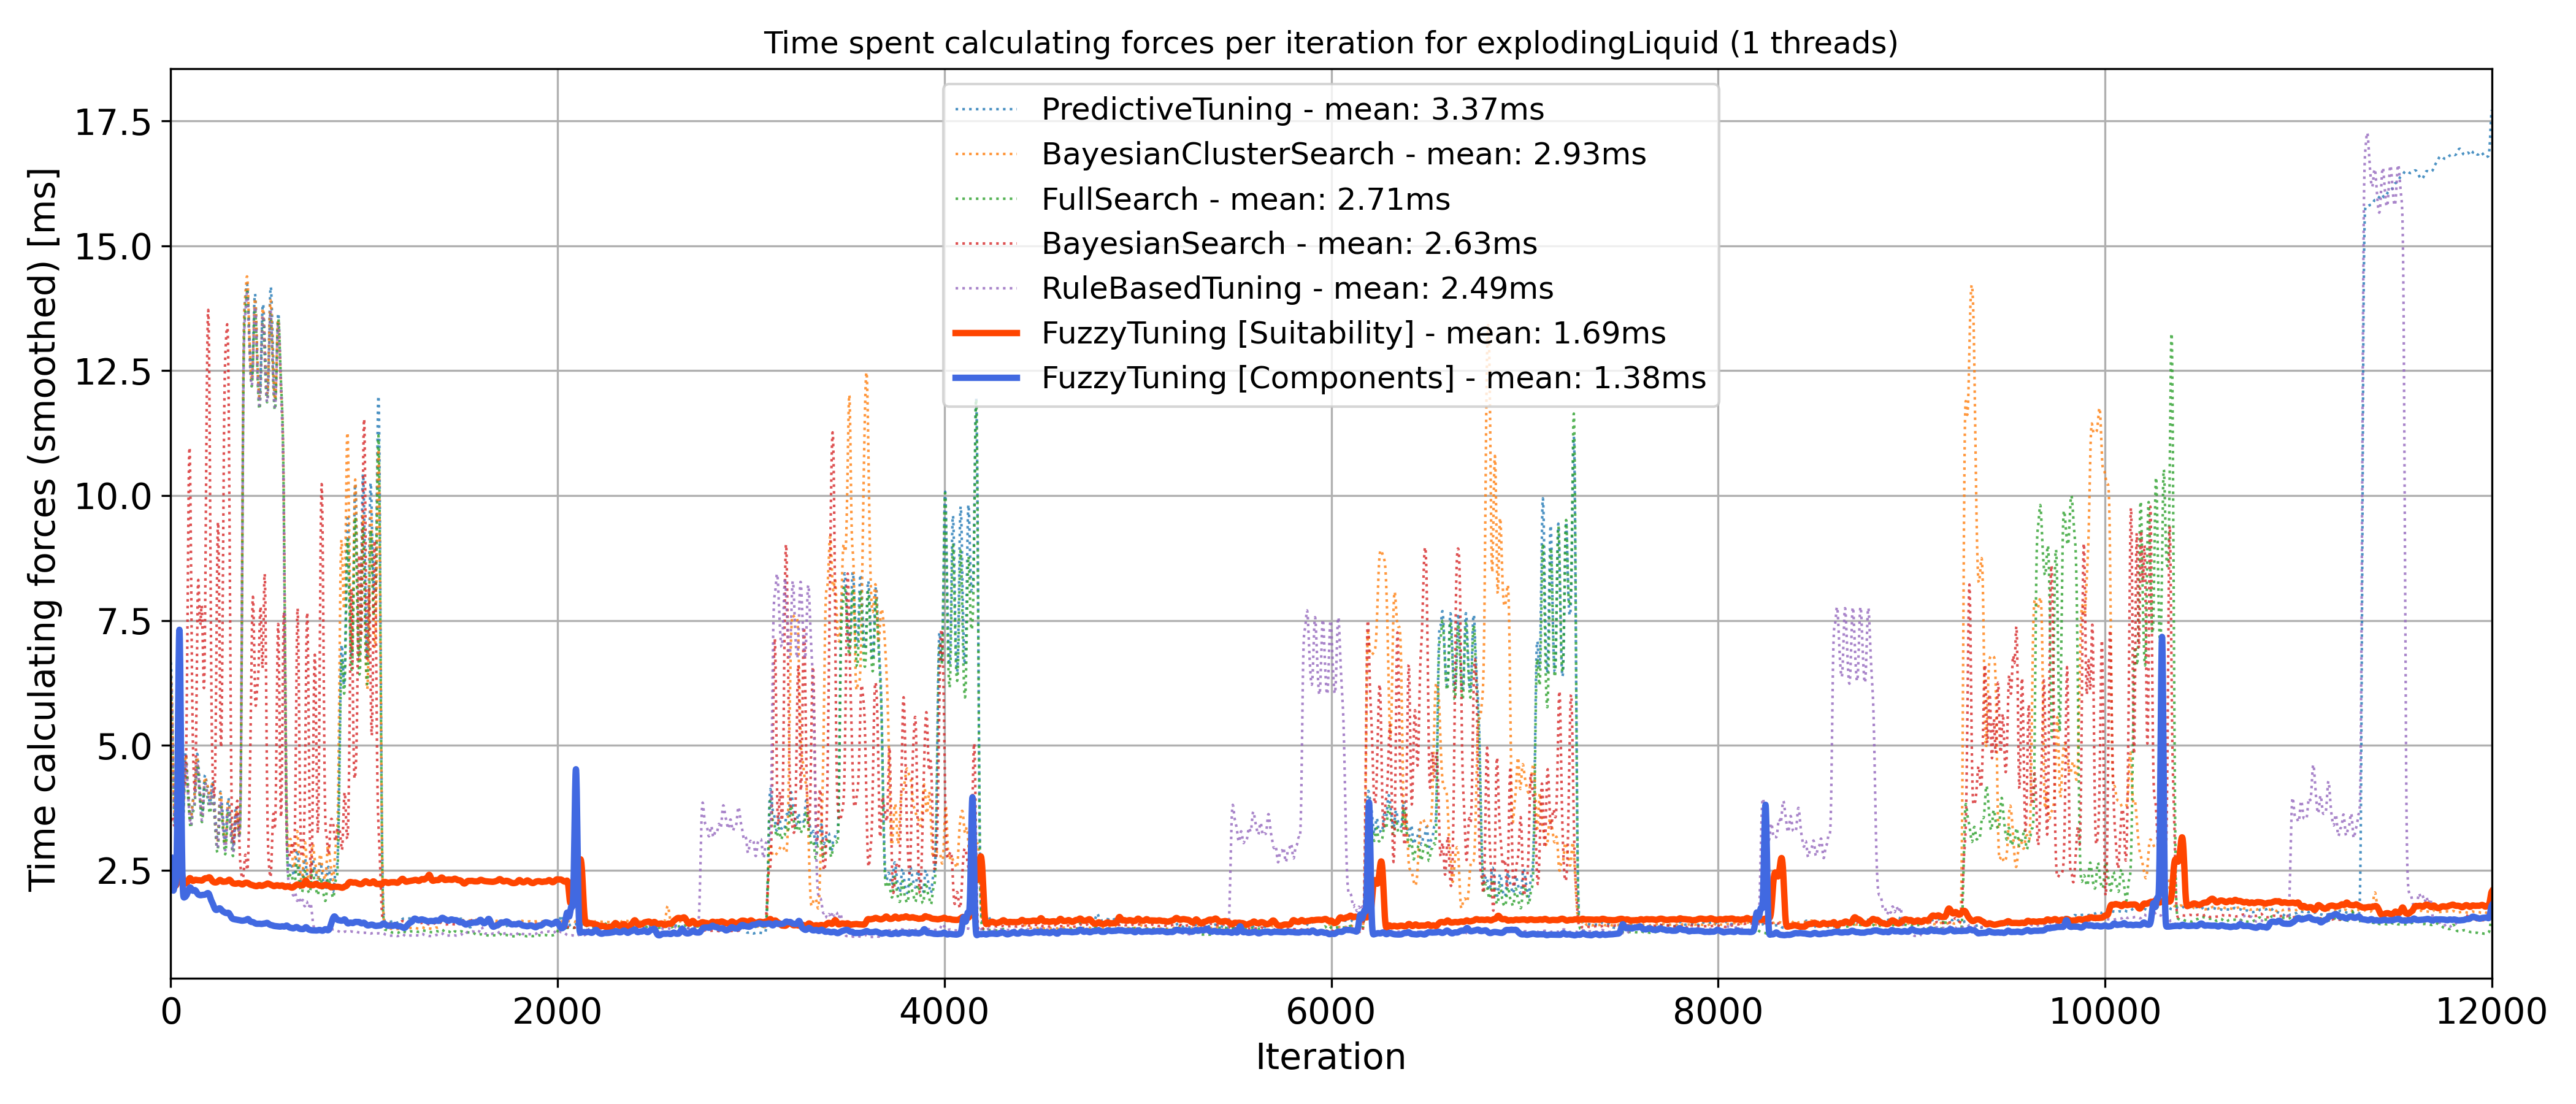
\includegraphics[width=\columnwidth,trim={0cm 0 0cm 0.9cm},clip]{figures/Benchmark/ExplodingLiquid/timing_explodingLiquid_1.png}
        \caption{}
        \label{fig:explodingTimings_1thread}
    \end{subfigure}


    \begin{subfigure}[c]{\textwidth}
        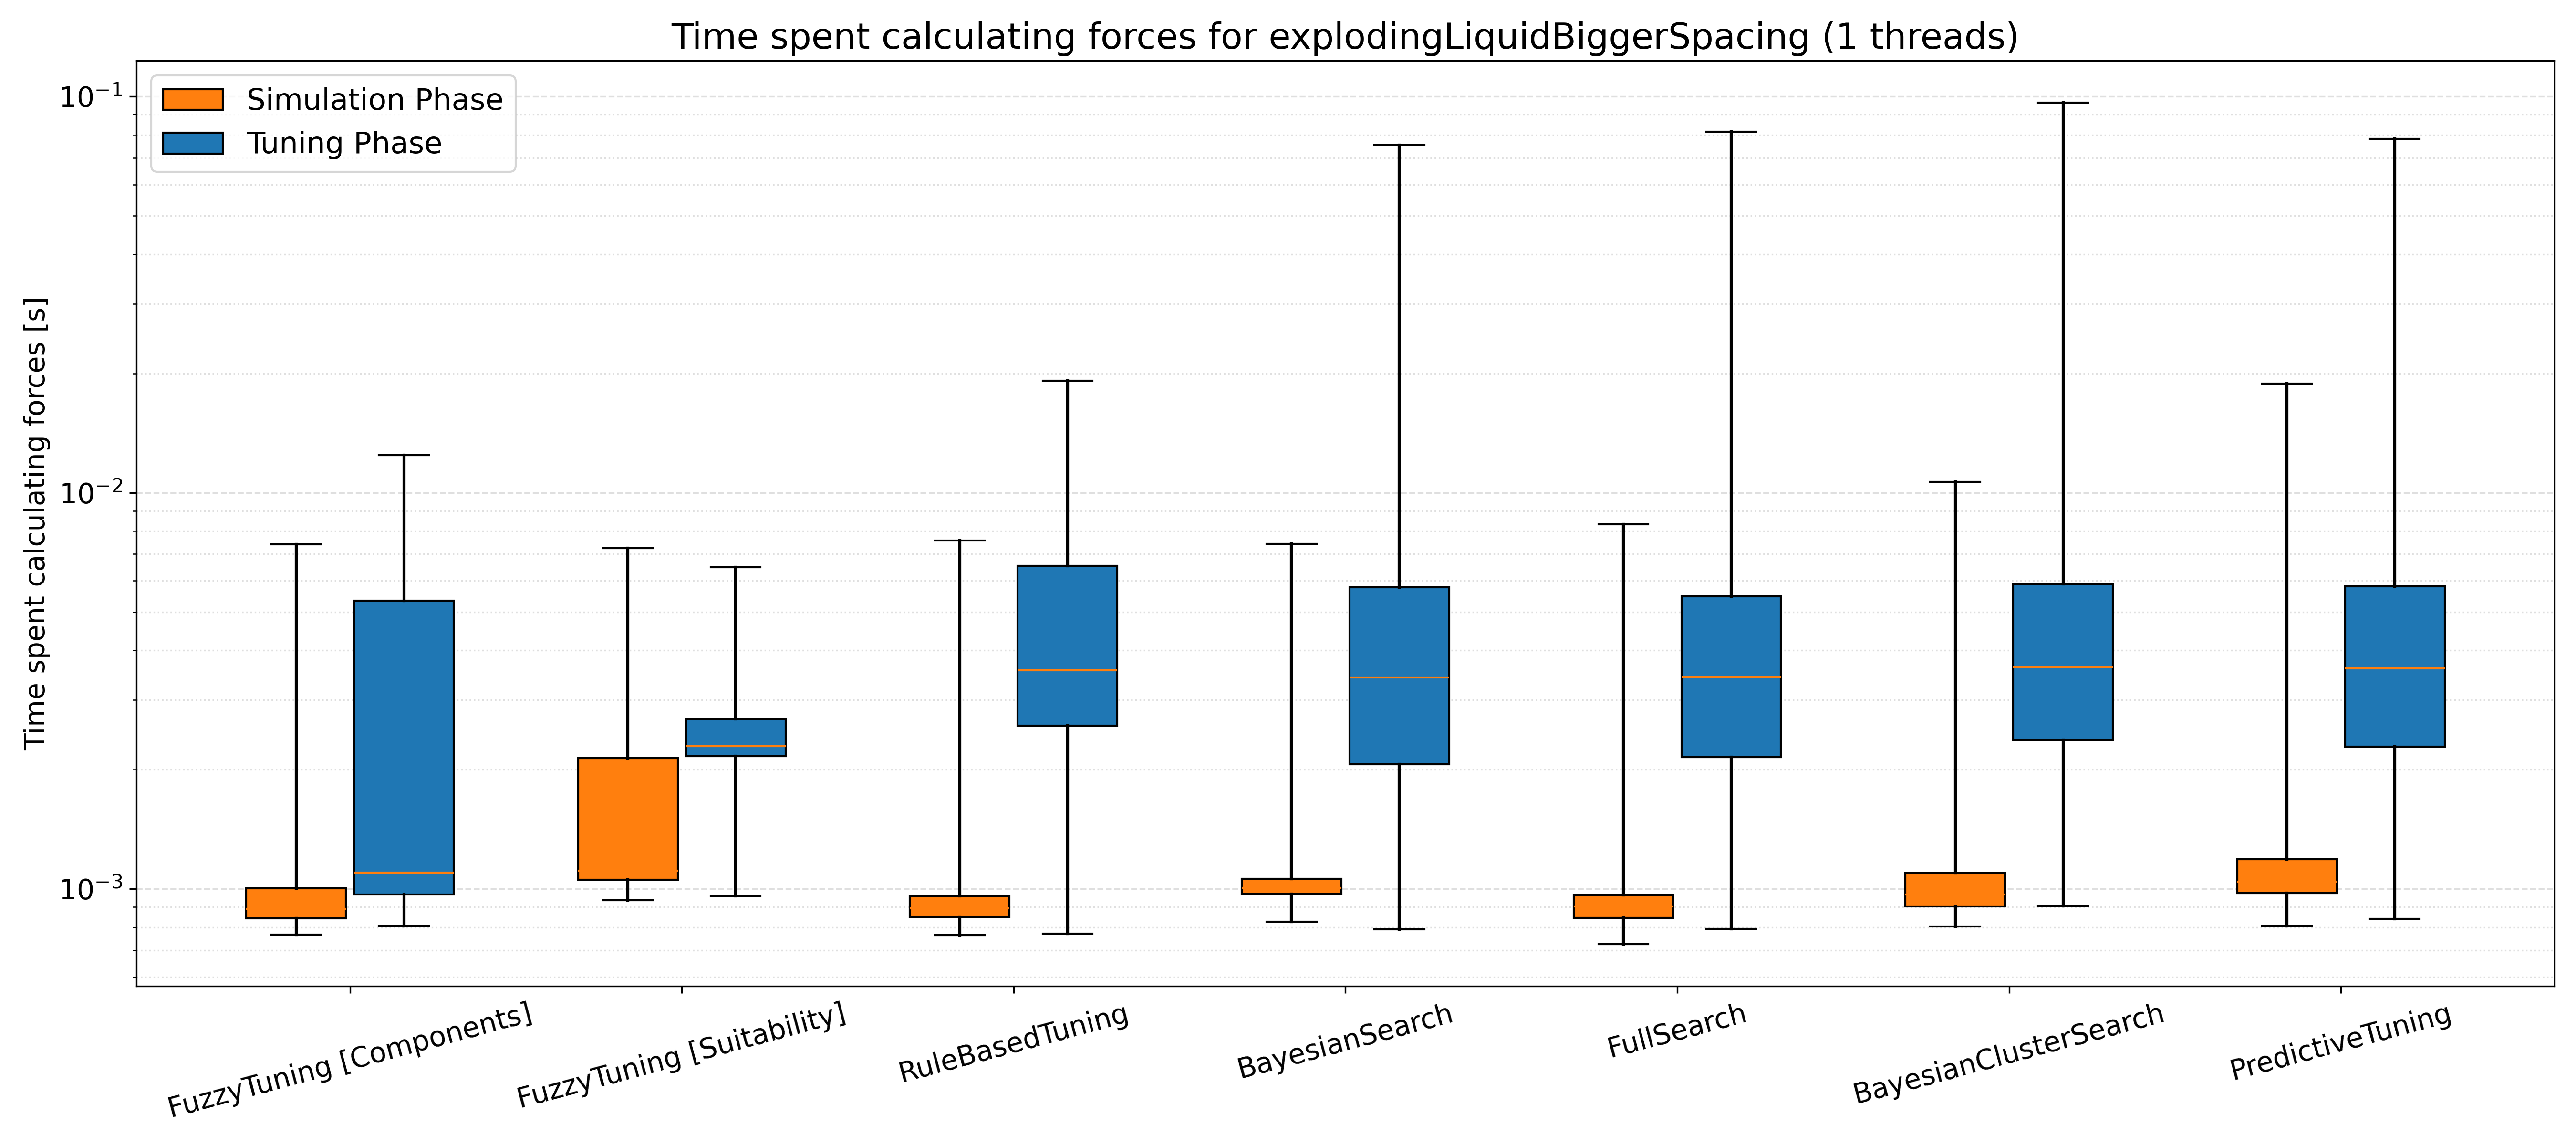
\includegraphics[width=\columnwidth,trim={0cm 0 0cm 1cm},clip]{figures/Benchmark/ExplodingLiquid/boxplot_explodingLiquid_1.png}
        \caption{}
        \label{fig:explodingLiquidBoxplot_1thread}
    \end{subfigure}

    \begin{subfigure}[b]{\textwidth}
        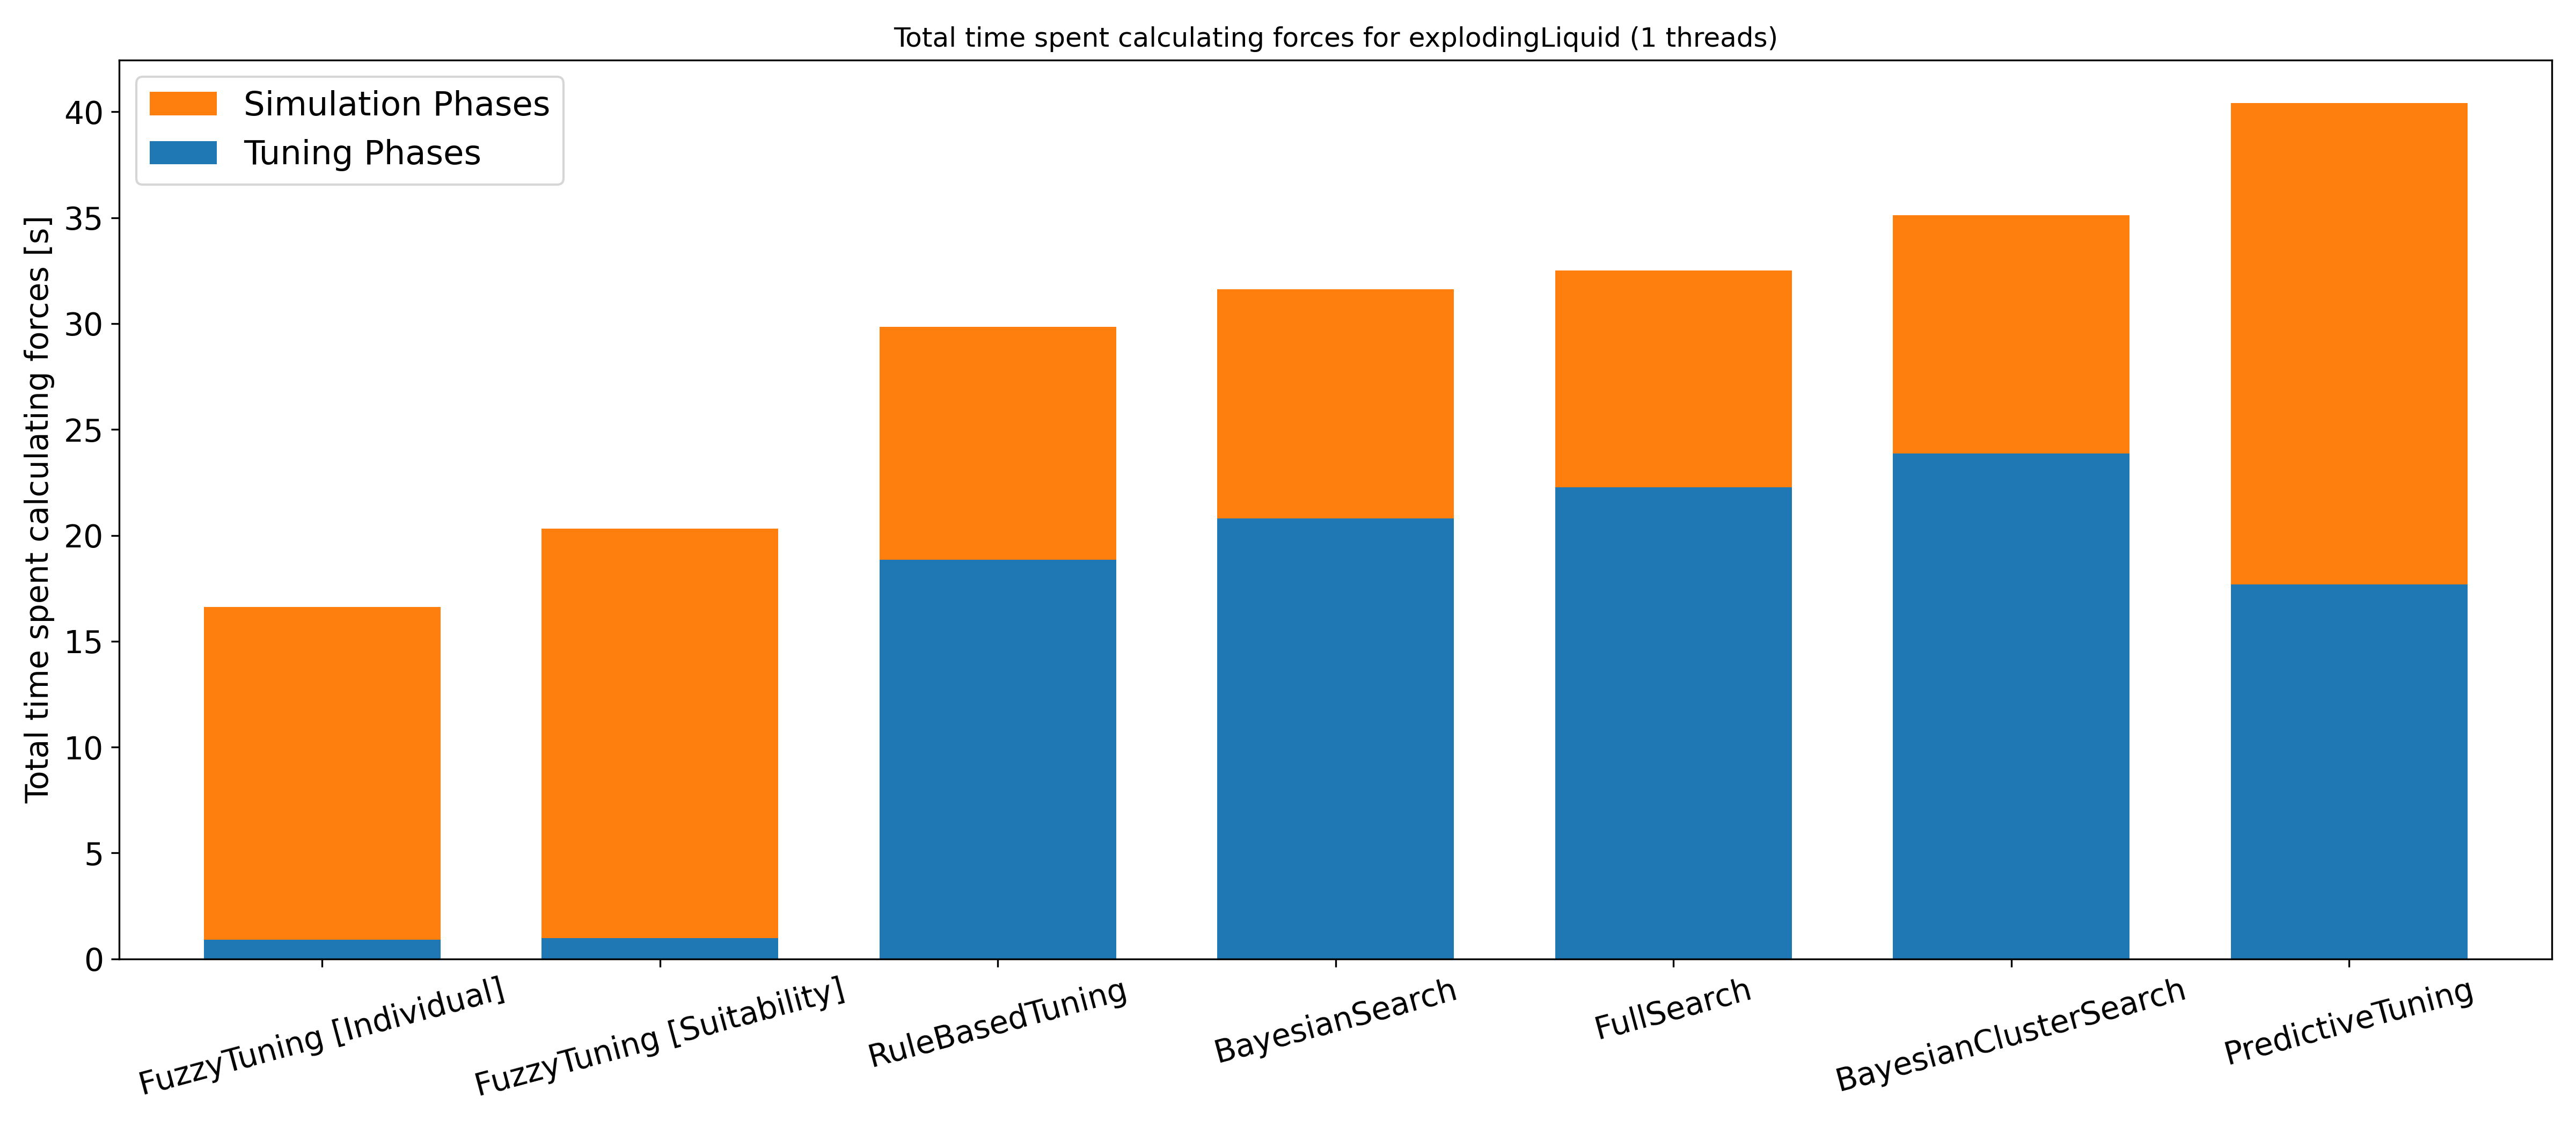
\includegraphics[width=\columnwidth,trim={0cm 0 0cm 0.9cm},clip]{figures/Benchmark/ExplodingLiquid/total_time_explodingLiquid_1.png}
        \caption{}
        \label{fig:explodingLiquidTotalTime_1thread}
    \end{subfigure}


    \caption[Exploding liquid benchmark with 1 thread]{Exploding liquid benchmark with 1 thread. (a) Time spent calculating forces. (b) Boxplots of time spent calculating forces divided into simulation and tuning phases. (c) Total time spent calculating forces}
    \label{fig:explodingLiquid_1thread}
\end{figure}

\begin{figure}[H]
    \centering

    \begin{subfigure}[c]{\textwidth}
        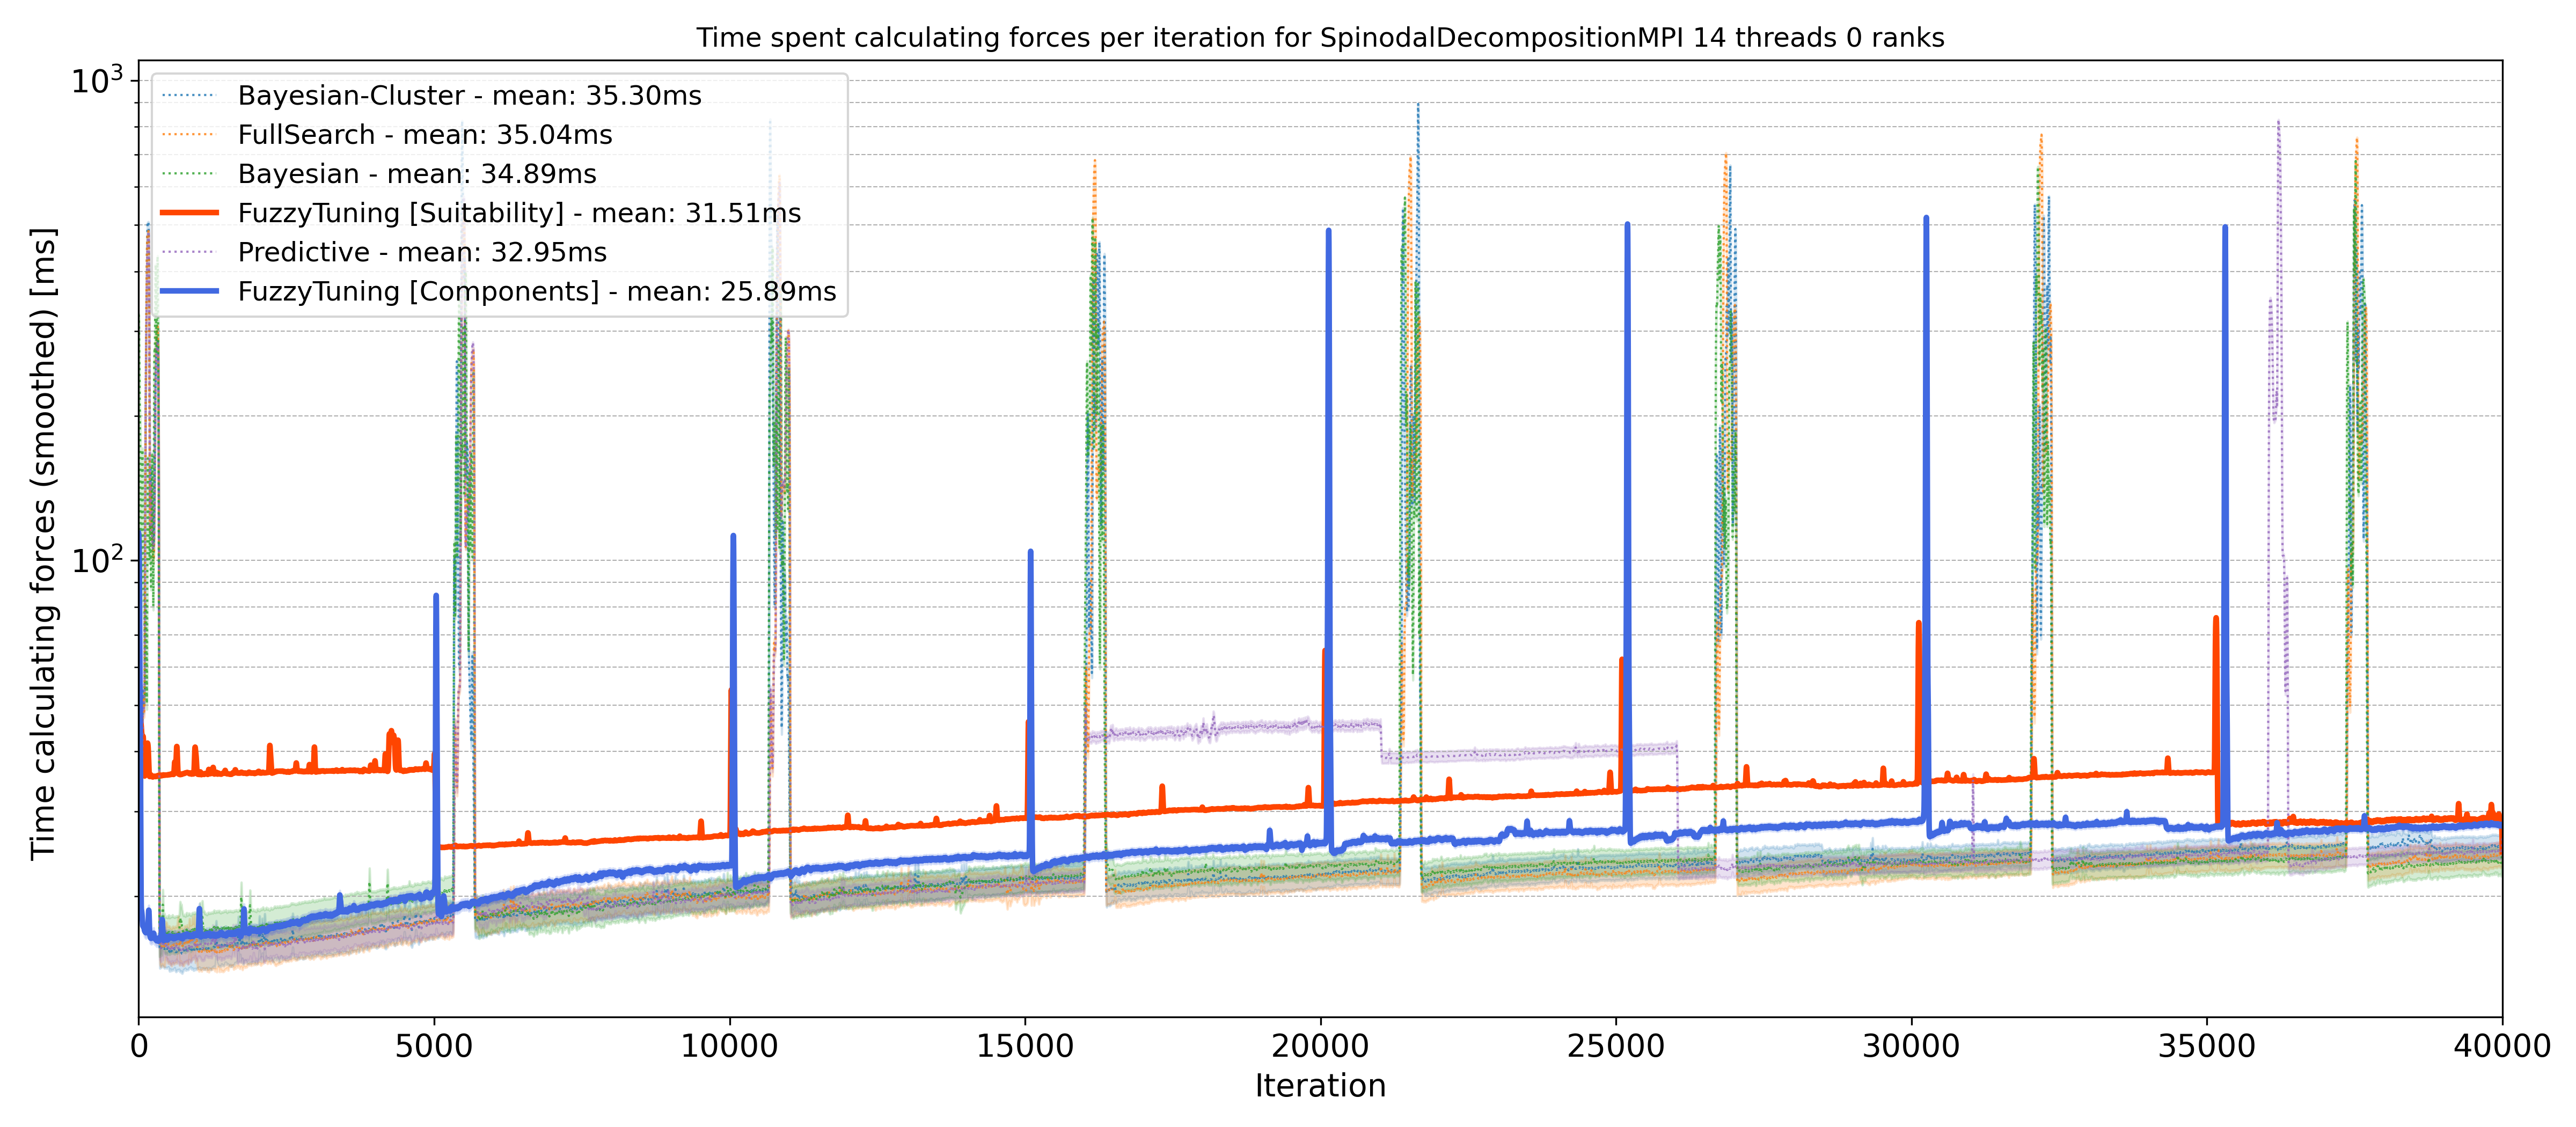
\includegraphics[width=\columnwidth,trim={0cm 0 0cm 0.9cm},clip]{figures/Benchmark/SpinodalDecompositionMPI/SpinodalDecompositionMPI_timings_SpinodalDecompositionMPI_14_0.png}
        \caption{}
        \label{fig:spinodalTimings_14thread}
    \end{subfigure}


    \begin{subfigure}[c]{\textwidth}
        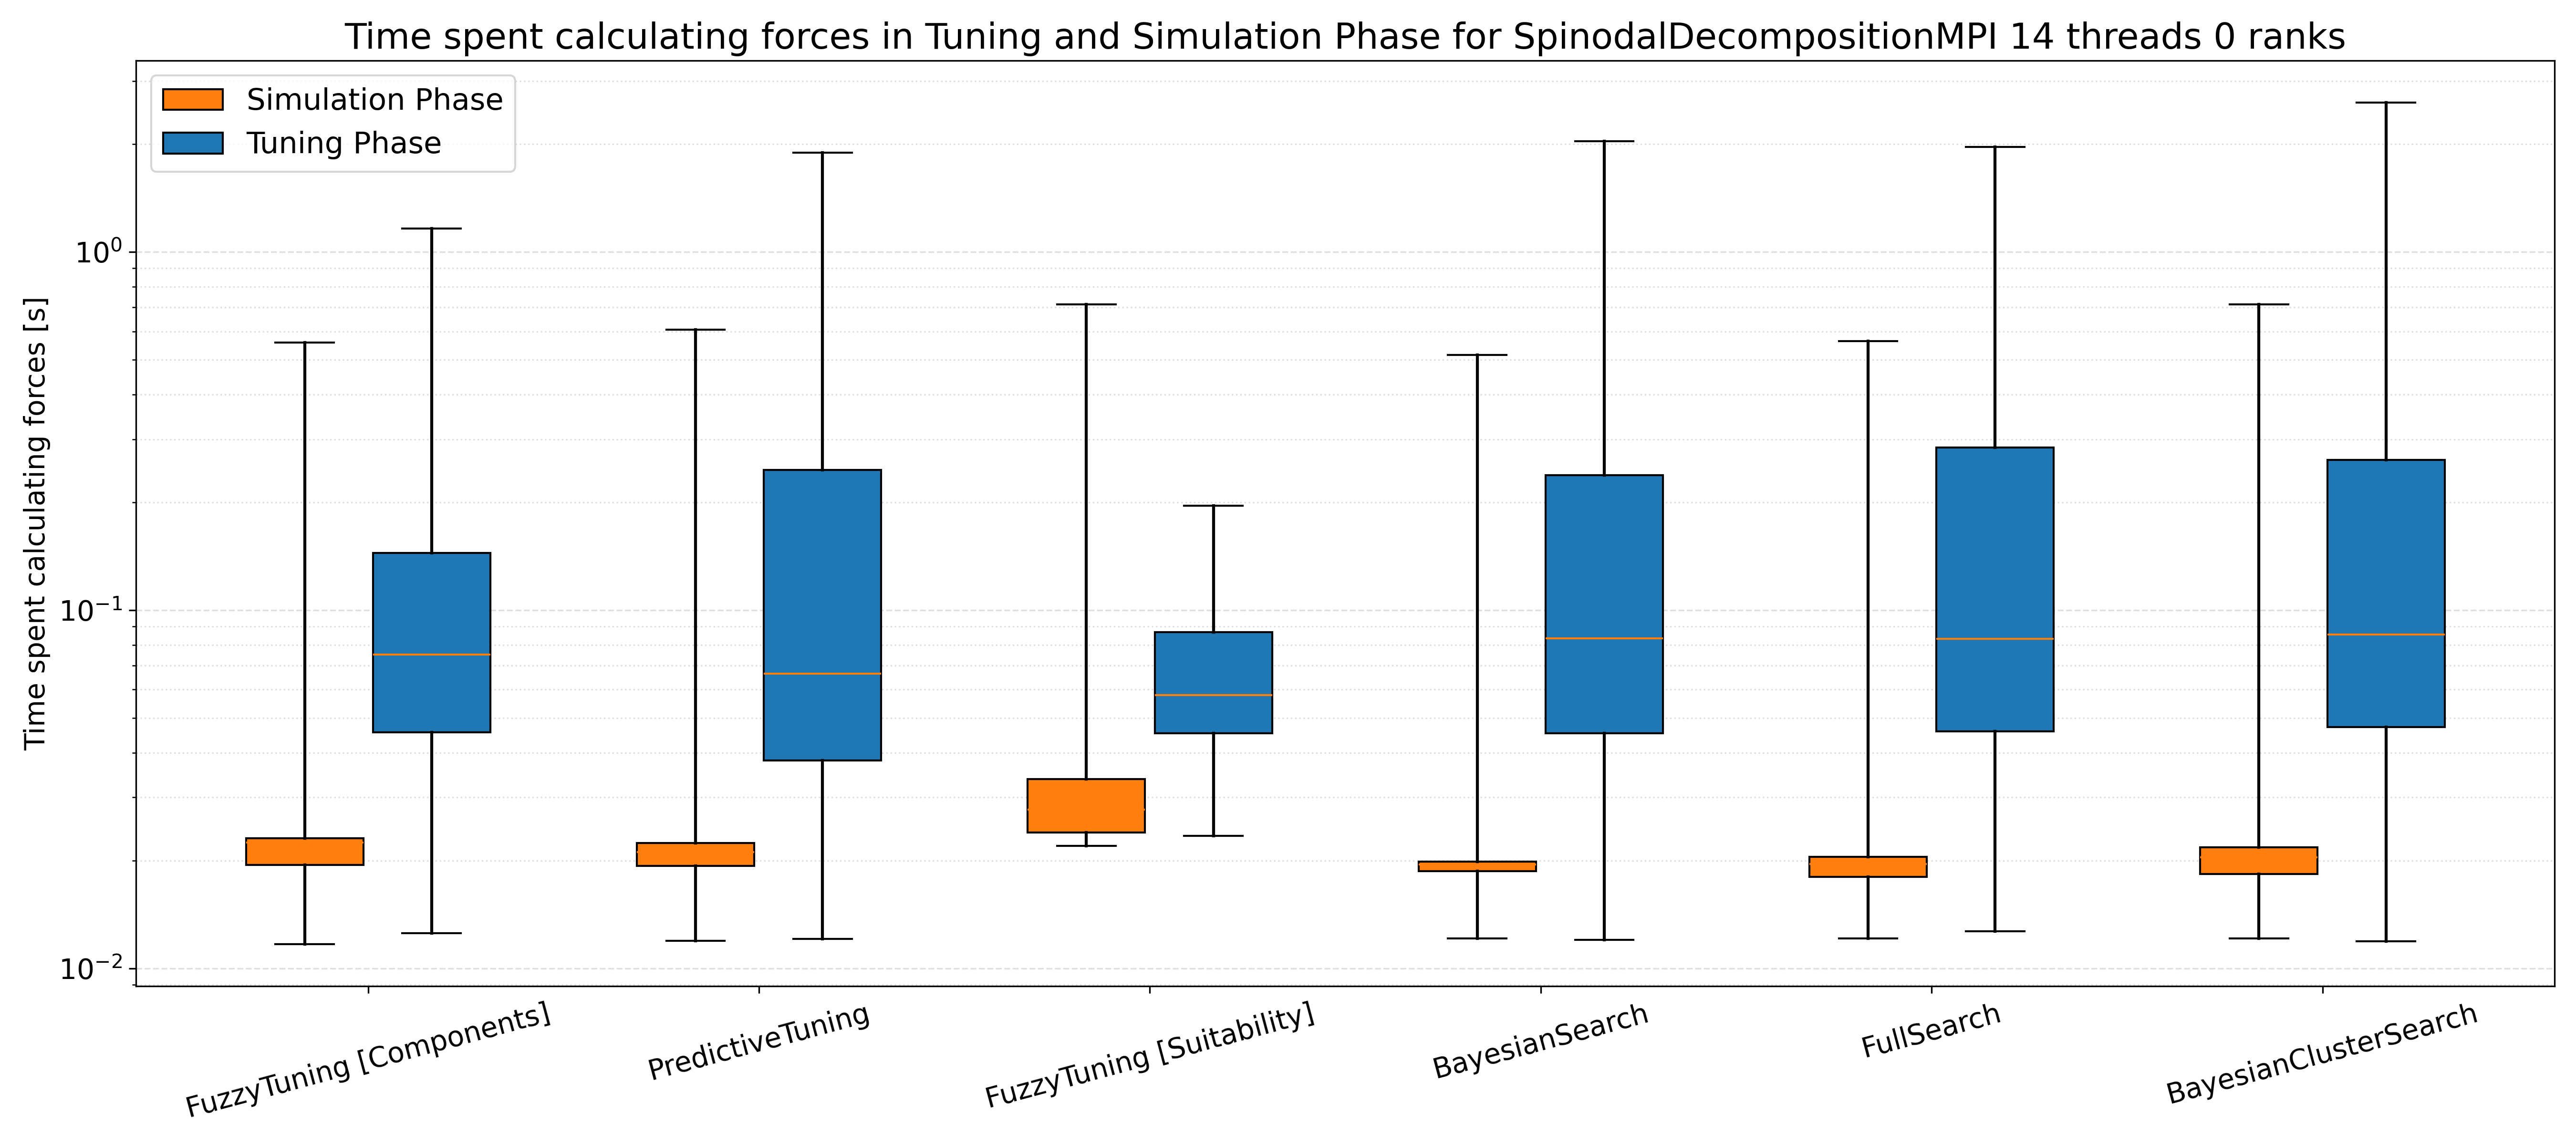
\includegraphics[width=\columnwidth,trim={0cm 0 0cm 1cm},clip]{figures/Benchmark/SpinodalDecompositionMPI/SpinodalDecompositionMPI_timings_boxplot_SpinodalDecompositionMPI_14_0.png}
        \caption{}
        \label{fig:spinodalBoxplot_14thread}
    \end{subfigure}

    \begin{subfigure}[b]{\textwidth}
        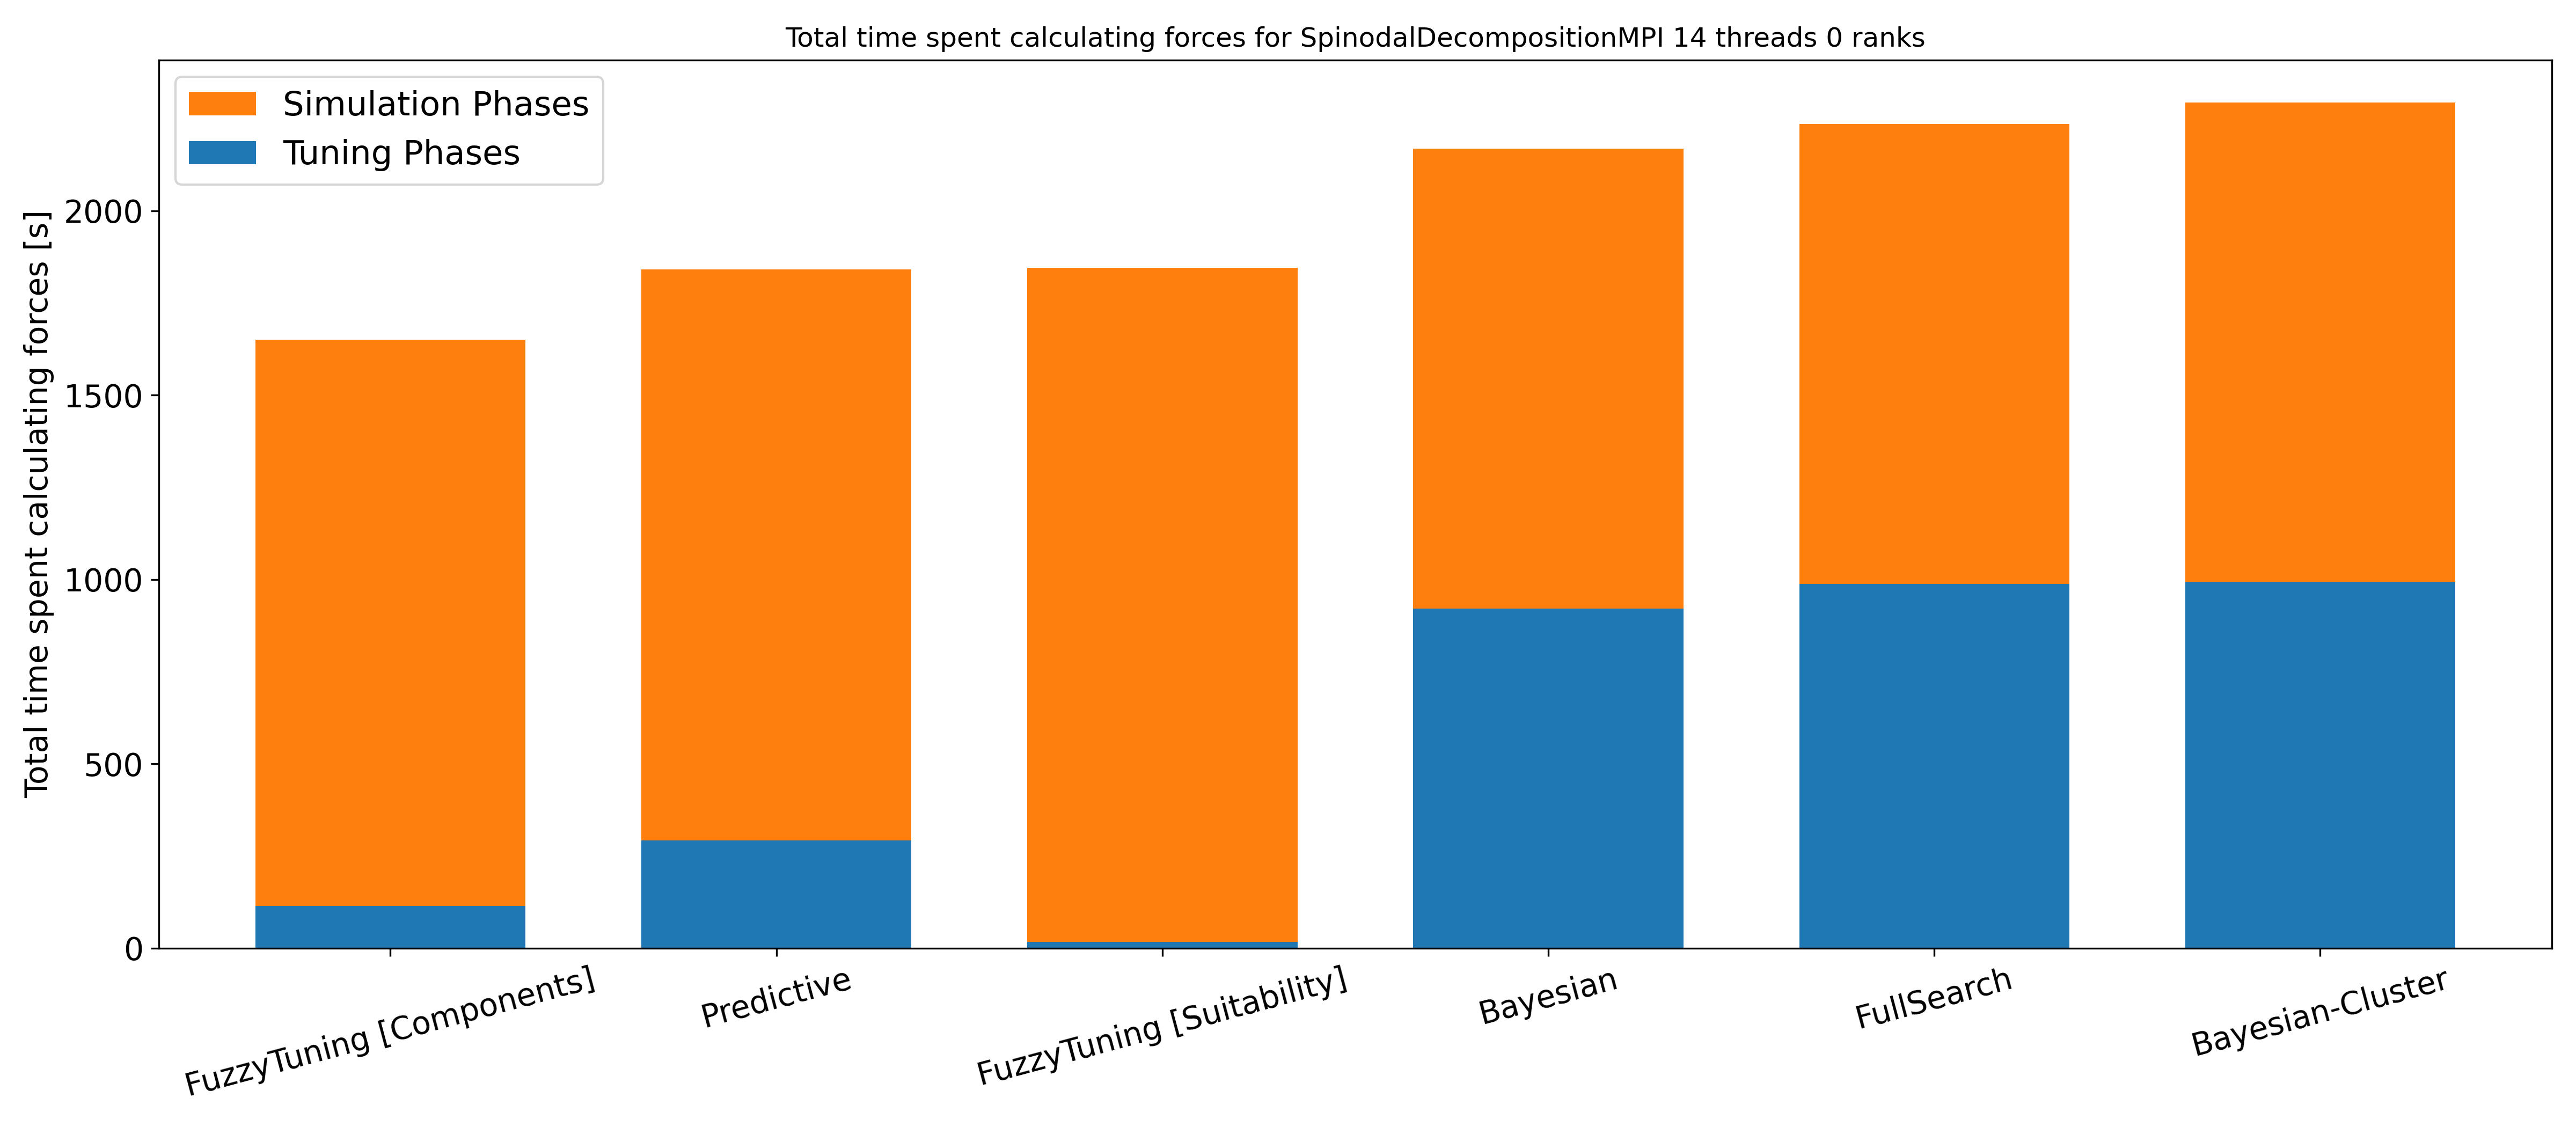
\includegraphics[width=\columnwidth,trim={0cm 0 0cm 0.9cm},clip]{figures/Benchmark/SpinodalDecompositionMPI/SpinodalDecompositionMPI_timings_total_SpinodalDecompositionMPI_14_0.png}
        \caption{}
        \label{fig:spinodalTotalTime_14thread}
    \end{subfigure}


    \caption[Spinodal decomposition benchmark MPI with 14 threads]{0th Rank of the Spinodal decomposition benchmark (Total: 4 MPI ranks, 14 threads each). (a) Time spent calculating forces. (b) Boxplots of time spent calculating forces divided into simulation and tuning phases. (c) Total time spent calculating forces}
    \label{fig:spinodal_14thread}
\end{figure}



\subsection{General Observations}

As described above, a tremendous slowdown of the classical tuning strategies is caused by very bad configurations that are sometimes encountered during the tuning phases. To further illustrate this, we will investigate the speedup density distribution of all configurations evaluated during the tuning phases of the different strategies. In particular, we will look at the Exploding Liquid and Spinodal Decomposition MPI scenarios described above, as they represent \emph{small} and \emph{large} scenarios, respectively.

The plots in \autoref{fig:tuningPhaseSpeedup} show these relative speedup distributions. All non-rule-based tuning strategies tend to encounter configurations with extremely low speedups during the tuning phases. Some of those bad configurations are $\approx100$ times slower than the best configurations of the tuning phase. As seen in the previous plots, those very slow configurations completely ruin the performance of the classical tuning strategies during the tuning phases.

It is also interesting to note that most of those bad performances are caused by very slow Neighbour List rebuilds, especially in the Spinodal Decomposition MPI scenario. This means that tuning strategies with very short tuning phases, like the fuzzy tuning strategies, have a significant advantage, as they only tend to evaluate configurations expected to suit the current state.

In both scenarios, the fuzzy tuning strategies have the best speedup distributions and, by far, the highest mean speedup during the tuning phases. However, this does not automatically mean they will perform their best in the following simulation phase, as they could fail to predict the optimal configuration.

\newpage

\begin{figure}[H]
    \centering

    \begin{subfigure}[c]{\textwidth}
        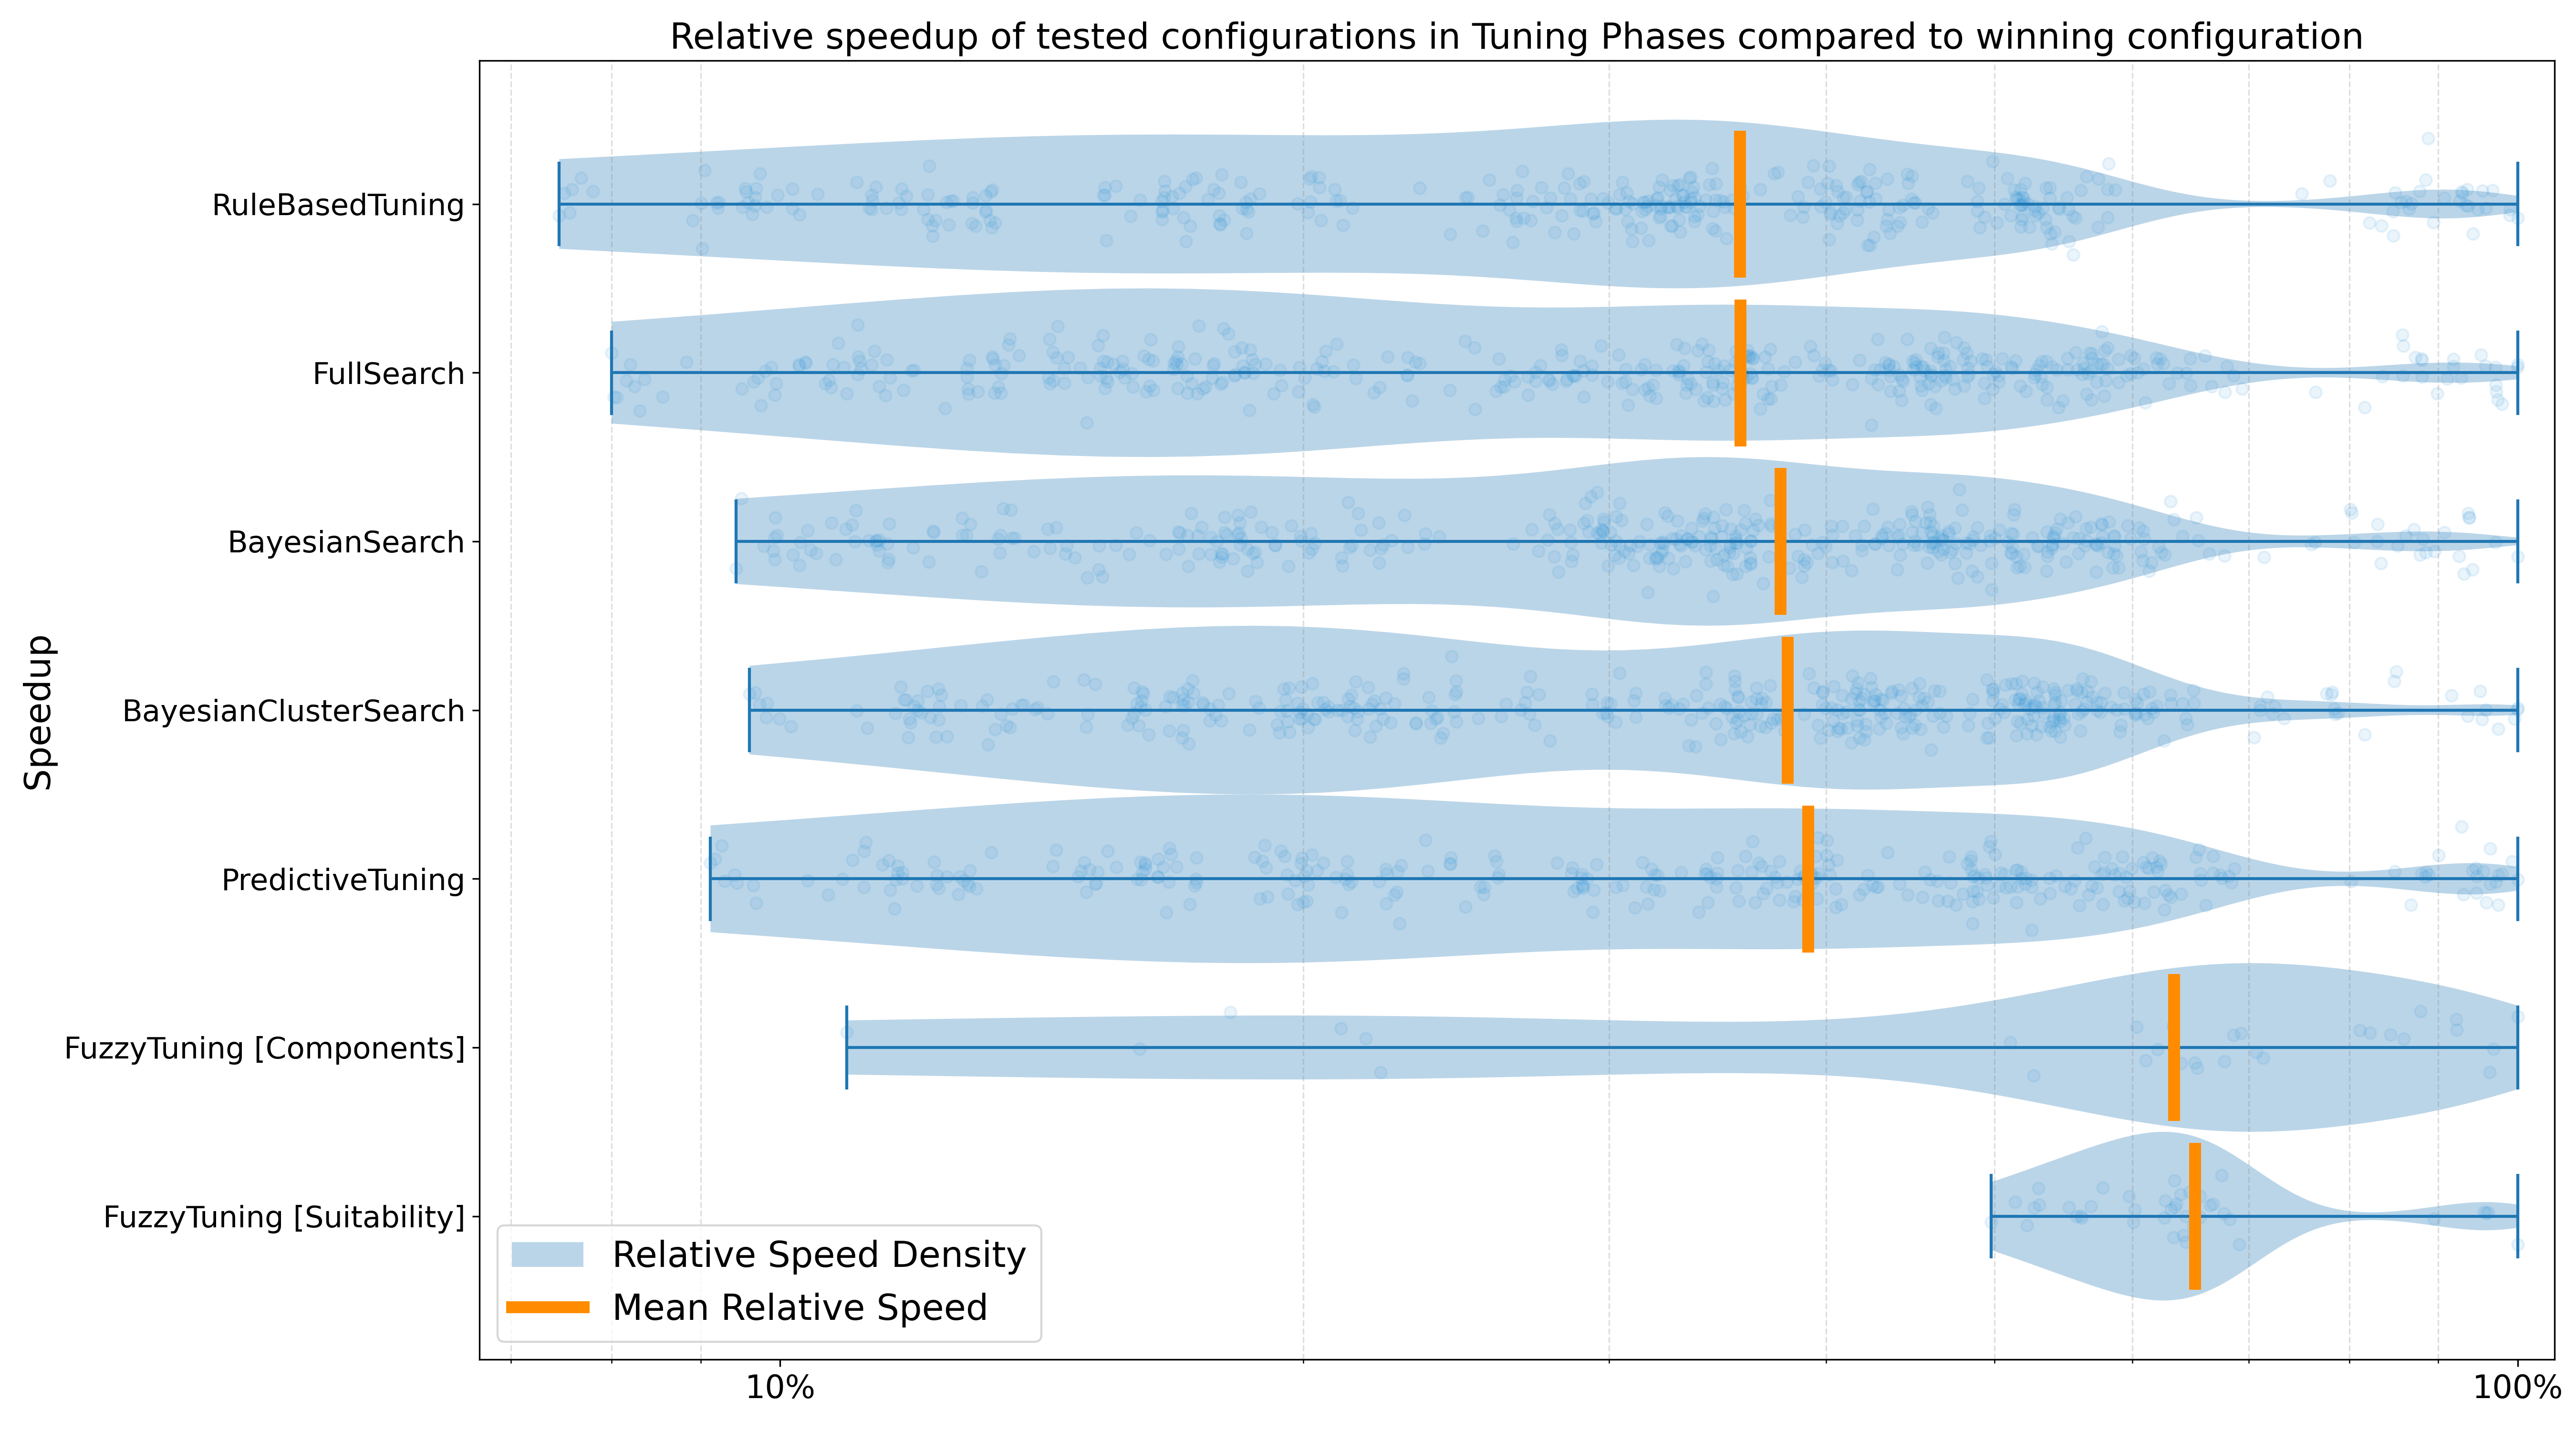
\includegraphics[width=\columnwidth,trim={1cm 0 0cm 1cm},clip]{figures/Benchmark/Observations/tuning_phase_speedup_explodingLiquid_1_zoomed.png}
        \caption{Exploding Liquid scenario with one thread.}
        \label{fig:explodingLiquidSpeedupDensity}
    \end{subfigure}


    \begin{subfigure}[c]{\textwidth}
        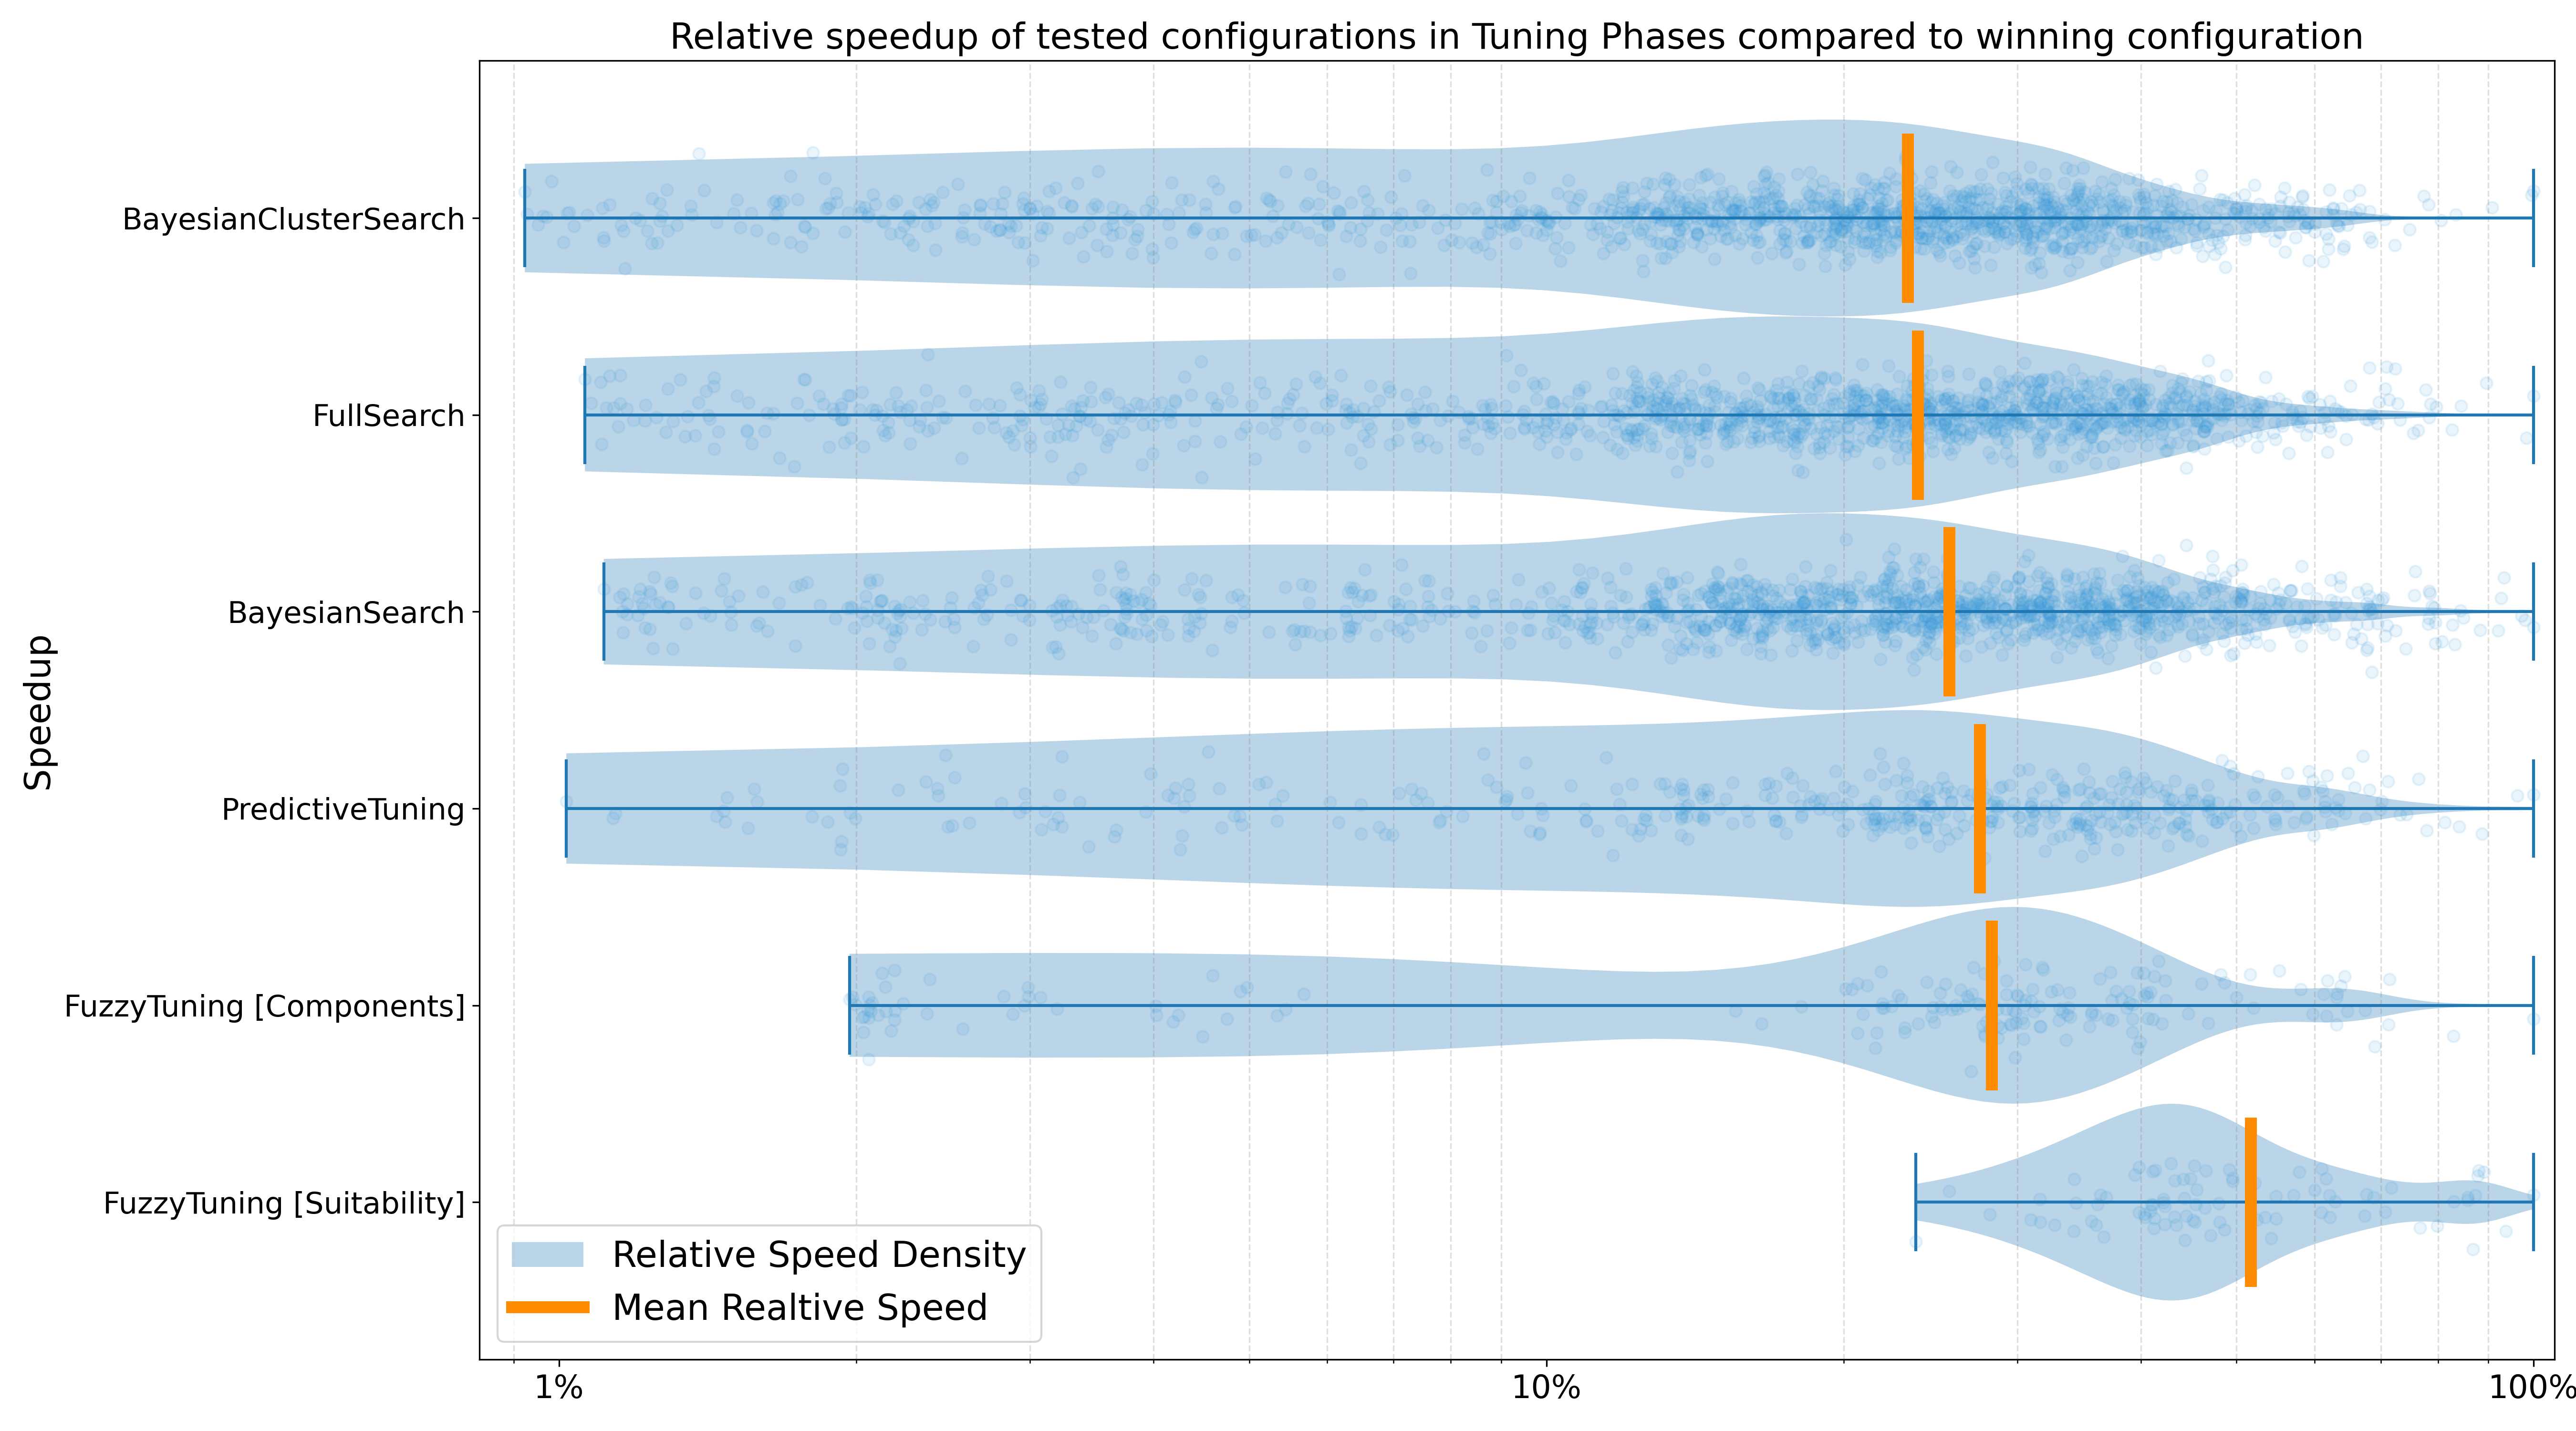
\includegraphics[width=\columnwidth,trim={1cm 0 0cm 1cm},clip]{figures/Benchmark/Observations/tuning_phase_speedup_SpinodalDecompositionMPI_14_0.png}
        \caption{Rank 0 of the Spinodal Decomposition MPI scenario with 14 threads.}
        \label{fig:spinodalSpeedupDensity}
    \end{subfigure}


    \caption[Quality of predictions during tuning phases]{The plot shows the speedup density distribution of all configurations evaluated during the tuning phases of both the Exploding Liquid and Spinodal Decomposition MPI scenarios. Most slow configurations are caused by the very slow Neighbour List rebuilds, especially in the Spinodal Decomposition MPI scenario, as there are many more particles.}
    \label{fig:tuningPhaseSpeedup}
\end{figure}


\begin{figure}
    \centering
    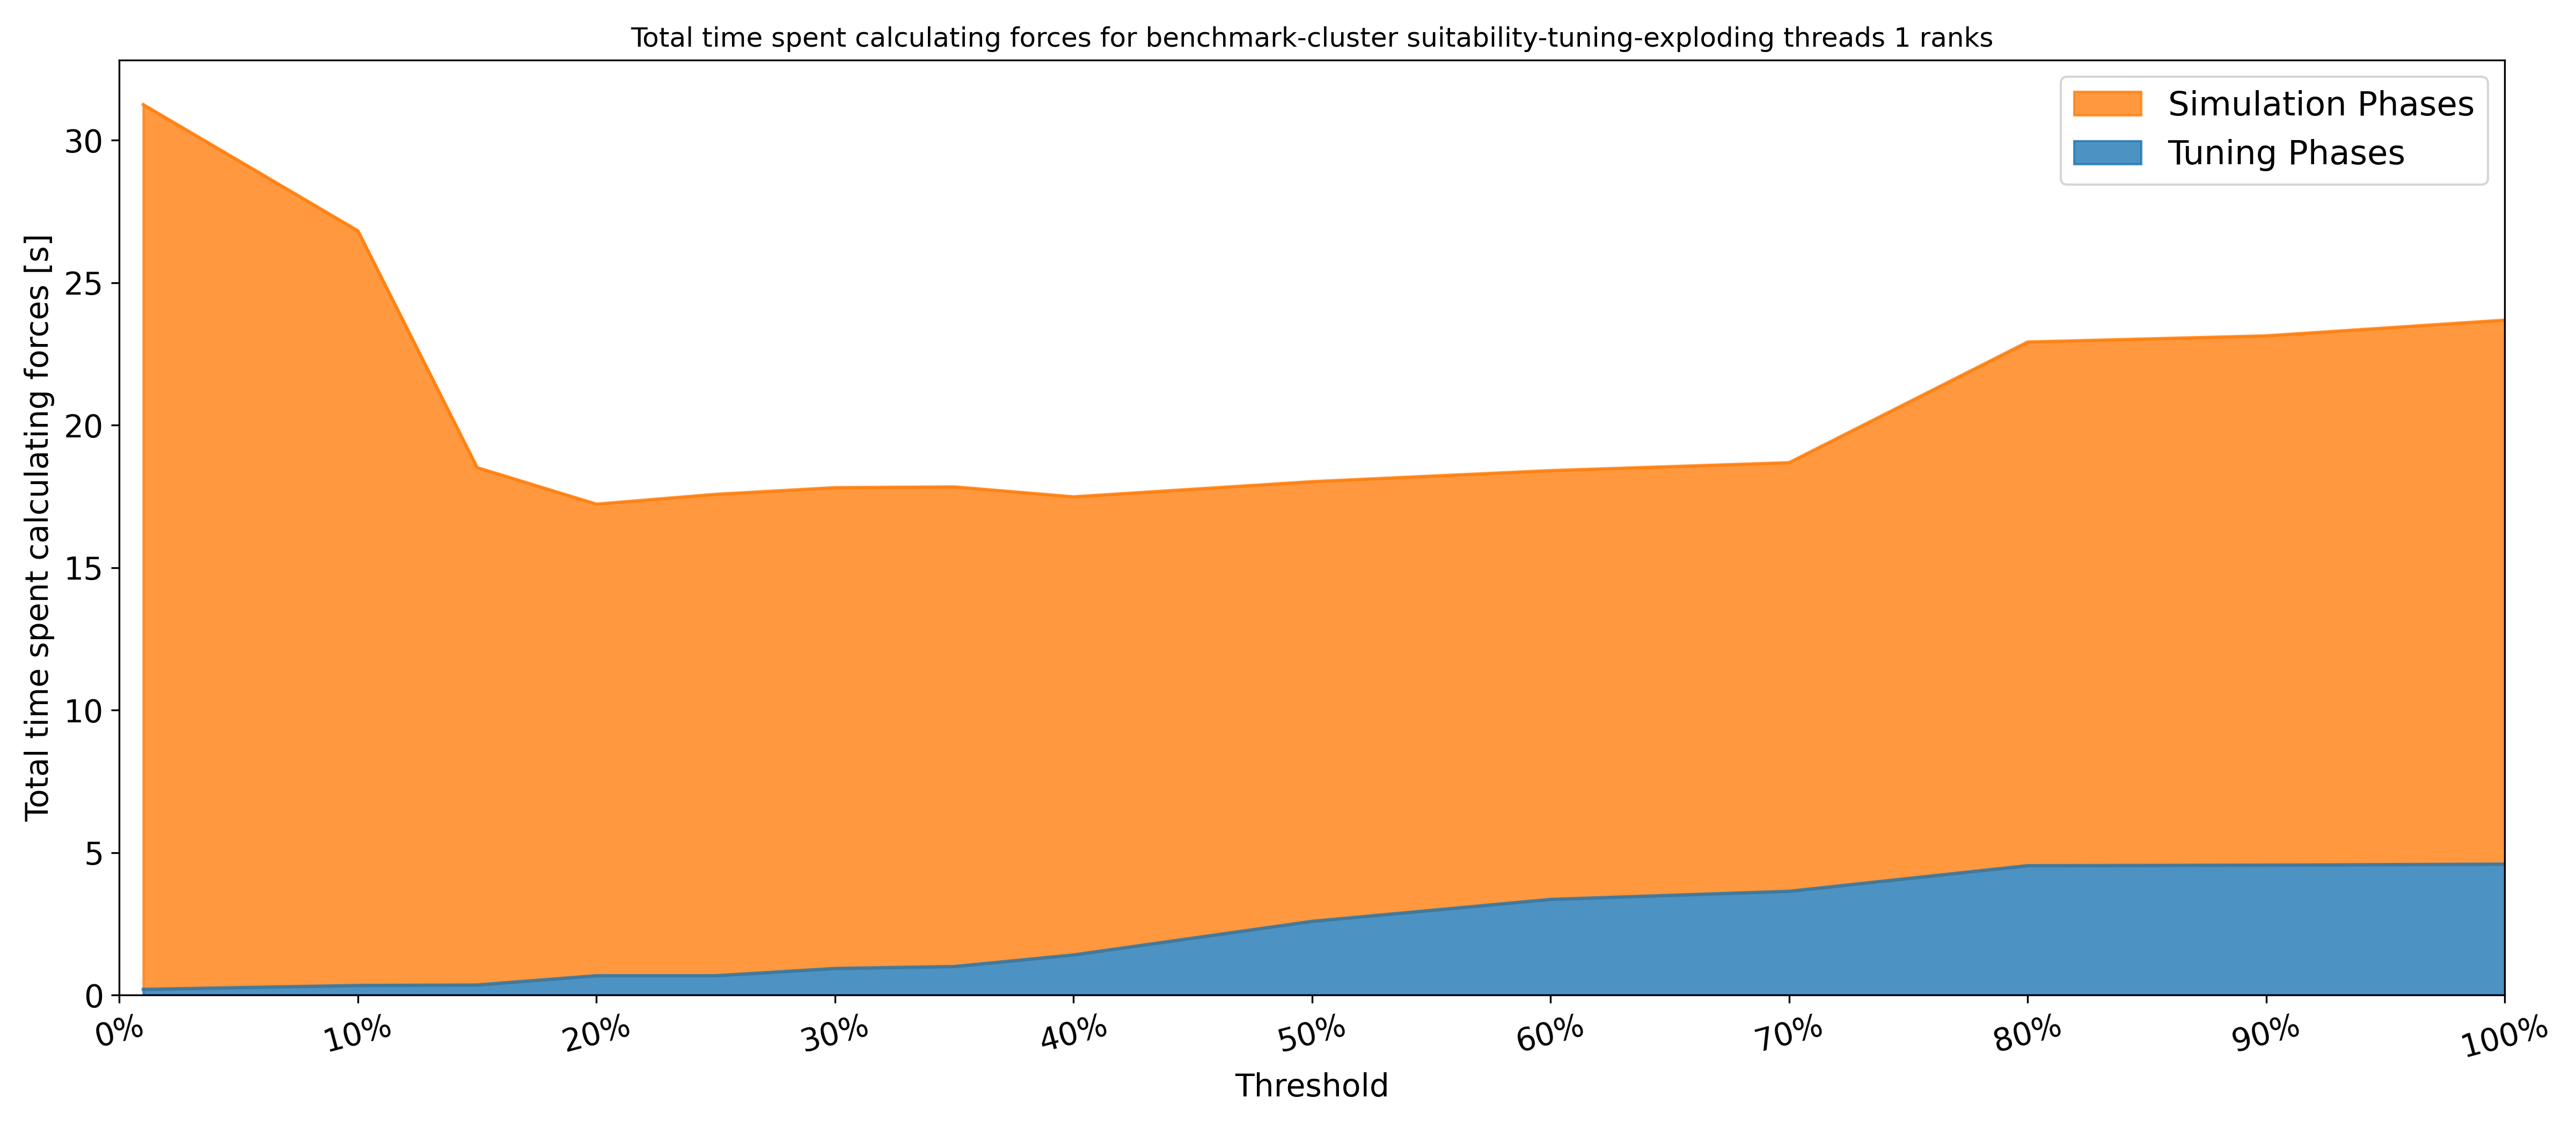
\includegraphics[width=\columnwidth]{figures/Benchmark/SuitabilitySearch/SuitabilityExploding_timings_threshold_benchmark-cluster_suitability-tuning-exploding_1.png}
    \caption[Exploding liquid benchmark with different suitability thresholds]{Exploding liquid benchmark with different suitability thresholds. The suitability threshold specifies the width of the interval around the best configuration, which determines how many configurations are selected for the tuning phase. Very low thresholds perform poorly, as they leave no margin for error and fail to select the best configuration. Very high thresholds also perform poorly, as high suitability values cause the strategy to behave like FullSeach. The optimal threshold for this scenario is between 20\% and 40\%.}
    \label{fig:suitabilityThreshold}
\end{figure}